% !TEX TS-program = pdflatex
% !TEX encoding = UTF-8 Unicode

\documentclass[11pt]{article} % use larger type; default would be 10pt

\usepackage[utf8]{inputenc} % set input encoding (not needed with XeLaTeX)

%%% PAGE DIMENSIONS
\usepackage{geometry} % to change the page dimensions
\geometry{margin=1in} % for example, change the margins to 2 inches all round

\usepackage{graphicx} % support the \includegraphics command and options

% \usepackage[parfill]{parskip} % Activate to begin paragraphs with an empty line rather than an indent

%%% PACKAGES
\usepackage[default]{cantarell}
\usepackage[T1]{fontenc}
\usepackage[none]{hyphenat}
\usepackage{booktabs} % for much better looking tables
\usepackage{bytefield}
\usepackage{array} % for better arrays (eg matrices) in maths
\usepackage{paralist} % very flexible & customisable lists (eg. enumerate/itemize, etc.)
\usepackage{verbatim} % adds environment for commenting out blocks of text & for better verbatim
\usepackage{subfig} % make it possible to include more than one captioned figure/table in a single float

%%% HEADERS & FOOTERS
\usepackage{fancyhdr} % This should be set AFTER setting up the page geometry
\pagestyle{fancy} % options: empty , plain , fancy
\lhead{RobotOpen Protocol Spec\\Version 1.0 (Jan 15th, 2012)\\www.RobotOpen.biz}
\rhead{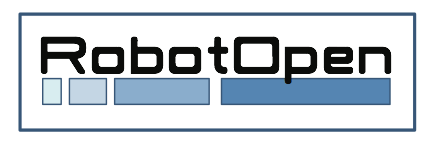
\includegraphics[height=42pt]{robotopen.png}}
\lfoot{}\cfoot{\thepage}\rfoot{}
\setlength\headsep{30pt}
\setlength\footskip{0pt}

\begin{document}

\section*{}

\section{Introduction}

\subsection{Overview}
The creation of the RobotOpen Protocol is an effort to design an open, standardized protocol for communication and control of hobbyist robots over an IP based network. It is designed for two-way communication and allows any arbitrary values to be bundled and transmitted.

\section{Protocol Structure}

\subsection{Data Bundles}
Data bundles are the primary method of grouping data together and transmitting it over the RobotOpen protocol. The payload of each packet is nothing more than each data bundle one after another. Data bundles are identified by a single character or ASCII byte. This is typically 0-9, a-z, or A-Z. By default, the Driver Station sends each joystick as its own data bundle. The first joystick has the bundle ID of '0', the second is '1' and so on. Each byte in these bundles corresponds to a joystick component (analog axis, button, etc...).

\subsection{Networking}
RobotOpen packets are typically transmitted as UDP over IP based networks, however there are no limitations on this. The RobotOpen Arduino library implements a UDP server listening on port 22211. The driver station or UDP client that wishes to connect to the robot sends RobotOpen packets to this port. The RobotOpen Arduino library will send all response packets to the high level port that is automatically assigned when the client connects to the server. Note that only one device or driver station should send packets to a robot controller at a time. This is not always enforced, so ensure that you have properly secured the network that your robot controller is connected to.

\subsection{Required Fields and Length}
Every RobotOpen packet must be at least 5 bytes long. This includes the message type, protocol version, device ID, and 16 bit CRC checksum. In this initial release, RobotOpen packets may not be longer than 256 bytes. This may change in future protocol revisions.

\subsection{Checksumming}
Because every RobotOpen packet has a 16 bit CRC, it is safe to assume that the data transmitted will not become corrupted in transit. Keep in mind that this does not guarantee the ordering of packets or even if the packet will ever be delivered.

\newpage

\section*{}
\section{Packet Types}
As stated earlier, every RobotOpen packet is required to have a packet type associated with it. This is always the first byte of each packet. There are currently 3 packet types, each listed below. Packet structures have been provided. The width of each box is assumed to be 8 bits or 1 byte.

\subsection{Control Packet}

Control packets are used for sending control data to a robot from a driver station. If a robot controller does not receive a control packet within 250ms of the last, it should automatically disable itself.
\vspace{30px}

\begin{bytefield}[bitformatting={\small\bfseries},bitwidth=24.0pt]{8}
\bitheader{0-7} \\
\bitbox{8}{Message Type} \\
\bitbox{8}{Protocol Version} \\
\bitbox{8}{Device ID} \\
\bitbox[lrt]{8}{Payload (Bundles)} \\
\skippedwords \\
\bitbox{8}{CRC-16 High Byte} \\
\bitbox{8}{CRC-16 Low Byte}
\end{bytefield}
\\\\\\
\textbf{Message Type}: Always 0x01 for control packets.\\\\
\textbf{Protocol Version}: The version of RobotOpen protocol. Currenly only version 1 exists. This is transmitted as 0x01. If a controller detects a version mismatch it should throw out the packet.\\\\
\textbf{Device ID}: Used to identify what device is sending control packets (Driver Station app, Android, iPhone, etc...). See the Device ID section at the end of this document.\\\\
\textbf{Payload}: The actual control data to be sent. This will be in the form of bundles. See the Payload section later in this document. This portion of the packet is variable length.\\\\
\textbf{CRC-16 High/Low Byte}: A CRC-16 checksum of the entire packet, excluding these CRC-16 bytes. This 16 bit value should be transmitted as 2 bytes. The first byte in the packet is always the high byte, followed by the low byte. If a packet becomes corrupt it should be thrown out.\\

\newpage
\subsection*{}
\subsection{Query Packet}

Query packets are sent from a driver station to a robot controller to request a feedback packet. Think of this packet type like a control packet with no payload. No control data is being sent but we'd like to receive data from the robot and notify it of our IP and port.
\vspace{30px}

\begin{bytefield}[bitformatting={\small\bfseries},bitwidth=24.0pt]{8}
\bitheader{0-7} \\
\bitbox{8}{Message Type} \\
\bitbox{8}{Protocol Version} \\
\bitbox{8}{Device ID} \\
\bitbox{8}{CRC-16 High Byte} \\
\bitbox{8}{CRC-16 Low Byte}
\end{bytefield}
\\\\\\
\textbf{Message Type}: Always 0x03 for query packets.\\\\
\textbf{Protocol Version}: The version of RobotOpen protocol. Currenly only version 1 exists. This is transmitted as 0x01. If a controller detects a version mismatch it should throw out the packet.\\\\
\textbf{Device ID}: Used to identify what device is sending query packets (Driver Station app, Android, iPhone, etc...). See the Device ID section at the end of this document.\\\\
\textbf{CRC-16 High/Low Byte}: A CRC-16 checksum of the entire packet, excluding these CRC-16 bytes. This 16 bit value should be transmitted as 2 bytes. The first byte in the packet is always the high byte, followed by the low byte. If a packet becomes corrupt it should be thrown out.\\

\newpage
\subsection*{}
\subsection{Feedback Packet}

Feedback packets are sent from a robot controller to a driver station. They contain robot state information and any data that should be sent back for display or processing on the DS. When a driver station sends a packet to a robot controller it should save the IP and port that sent the packet. All feedback packets are then returned to this IP/port. For every control and query packet, a feedback packet should be sent back.
\vspace{30px}

\begin{bytefield}[bitformatting={\small\bfseries},bitwidth=24.0pt]{8}
\bitheader{0-7} \\
\bitbox{8}{Message Type} \\
\bitbox{8}{Protocol Version} \\
\bitbox{8}{Device ID} \\
\bitbox{8}{Firmware Version} \\
\bitbox{8}{Controller State} \\
\bitbox{8}{Uptime} \\
\bitbox[lrt]{8}{Payload (Bundles)} \\
\skippedwords \\
\bitbox{8}{CRC-16 High Byte} \\
\bitbox{8}{CRC-16 Low Byte}
\end{bytefield}
\\\\\\
\textbf{Message Type}: Always 0x02 for feedback packets.\\\\
\textbf{Protocol Version}: The version of RobotOpen protocol. Currenly only version 1 exists. This is transmitted as 0x01. If a controller detects a version mismatch it should throw out the packet.\\\\
\textbf{Device ID}: Used to identify what device is sending the feedback packet (Arduino, Computer, etc...). See the Device ID section at the end of this document.\\\\
\textbf{Firmware Version}: Used for identifying the version of your control code loaded onto a robot. This will typically be user provided. Values can range from 0x00 to 0xFF.\\\\
\textbf{Controller State}: The state of your robot (enabled or disabled). If the robot is disabled it should return 0x00. If it is enabled it should return 0xFF.\\\\
\newpage
\section*{}
\textbf{Uptime}: The time (in minutes) that the controller has been powered on for. Values can range from 0x00 to 0xFF. After 255 minutes, the controller can either keep this value at 255 or loop around. The Arduino library currently caps this at 255.\\\\
\textbf{Payload}: Any additional feedback data to be sent. This will be in the form of bundles. See the Payload section later in this document. This portion of the packet is variable length.\\\\
\textbf{CRC-16 High/Low Byte}: A CRC-16 checksum of the entire packet, excluding these CRC-16 bytes. This 16 bit value should be transmitted as 2 bytes. The first byte in the packet is always the high byte, followed by the low byte. If a packet becomes corrupt it should be thrown out.\\
\newpage


\section*{}

\section{Payload}

The payload of a packet is nothing more than each data bundle one after another. Below is an example of how this data is structured. Data bundles are open ended and can used in any way you choose. Typically each joystick is sent as its own bundle in a control packet and each sensor or reading is sent back as a bundle in a feedback packet. When using the publish functions in the Arduino library, every value passed is placed into its own bundle.
\vspace{30px}

\begin{bytefield}[bitformatting={\small\bfseries},bitwidth=26.0pt]{8}
\bitheader{0-7} \\
\bitbox{8}{First Bundle Length (bytes after length)} & \\
\bitbox{8}{First Bundle ID} \\
\wordbox{3}{Variable Length Bundle Bytes} \\
\bitbox[lrt]{8}{} \\
\skippedwords \\
\bitbox{8}{Last Bundle Length (bytes after length)} & \\
\bitbox{8}{Last Bundle ID} \\
\wordbox{3}{Variable Length Bundle Bytes} \\
\end{bytefield}
\\\\\\
\textbf{Bundle Length}: This byte specifies the length of the bundle excluding the length byte. A bundle that has 2 bytes of payload will have a length of 0x03 due to the bundle ID byte.\\\\
\textbf{Bundle ID}: A single ASCII character that identifies this bundle. Although this can be any value between 0x00 and 0xFF, it is encouraged to use printable characters such as 0-9, a-z, or A-Z.\\\\
\textbf{Variable Length Bundle Bytes}: The actual data. This can be in whatever format is most convenient to you. For joysticks, each byte is a component value (y axis, dpad, button), however the use of this is open ended. ASCII strings could even be sent in a bundle using this portion.\\\\
As seen in the diagram, each bundle follows one after another. Both the driver station and robot controller will parse out each of these bundles individually.
\newpage


\section*{}

\section{Device IDs}

The following device IDs have been assigned thus far. Note that driver stations begin at 0x01 counting up and robot controllers begin at 0xFF counting down.

\begin{itemize}
\item OFFICIAL\_JAVA\_DS - 0x01
\item OFFICIAL\_ANDROID\_APP - 0x02
\item OFFICIAL\_IPHONE\_APP - 0x03
\item ROBOTOPEN\_V1 - 0xFF
\end{itemize}

\end{document}
